\documentclass[border=10pt]{standalone}
\usepackage{pgfplots}
\pgfplotsset{compat=1.18}
\usepgfplotslibrary{colormaps}
\begin{document}
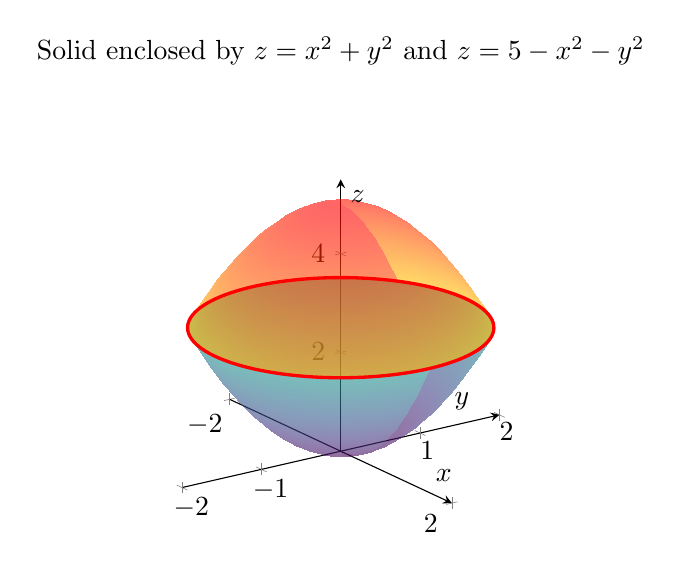
\begin{tikzpicture}
\begin{axis}[
    view={55}{25},
    axis lines=center,
    xlabel=$x$, ylabel=$y$, zlabel=$z$,
    xmin=-2, xmax=2, ymin=-2, ymax=2, zmin=0, zmax=5.5,
    title={Solid enclosed by $z=x^2+y^2$ and $z=5-x^2-y^2$},
    grid=major,
]
% lower paraboloid z = x^2+y^2 over disk r<=sqrt(5/2)
\addplot3[
    surf, shader=interp,
    colormap/viridis,
    domain=0:1.58113883, y domain=0:360,
    samples=25, samples y=50,
    opacity=0.6,
    trig format plots=deg,
    point meta=z,
]
({x*cos(y)}, {x*sin(y)}, {x^2});
% upper paraboloid z = 5 - x^2 - y^2 over same disk
\addplot3[
    surf, shader=interp,
    colormap/hot,
    domain=0:1.58113883, y domain=0:360,
    samples=25, samples y=50,
    opacity=0.6,
    trig format plots=deg,
    point meta=z,
]
({x*cos(y)}, {x*sin(y)}, {5-x^2});
% intersection circle
\addplot3[
    no markers, red, very thick,
    domain=0:360, samples=120, samples y=0,
    trig format plots=deg,
]
({1.58113883*cos(x)}, {1.58113883*sin(x)}, {2.5});
\end{axis}
\end{tikzpicture}
\end{document}
